\section{Implementation}
\label{section:implementation:architecture}
\subsection{Architecture}
    \begin{figure}[H]
        \centering
        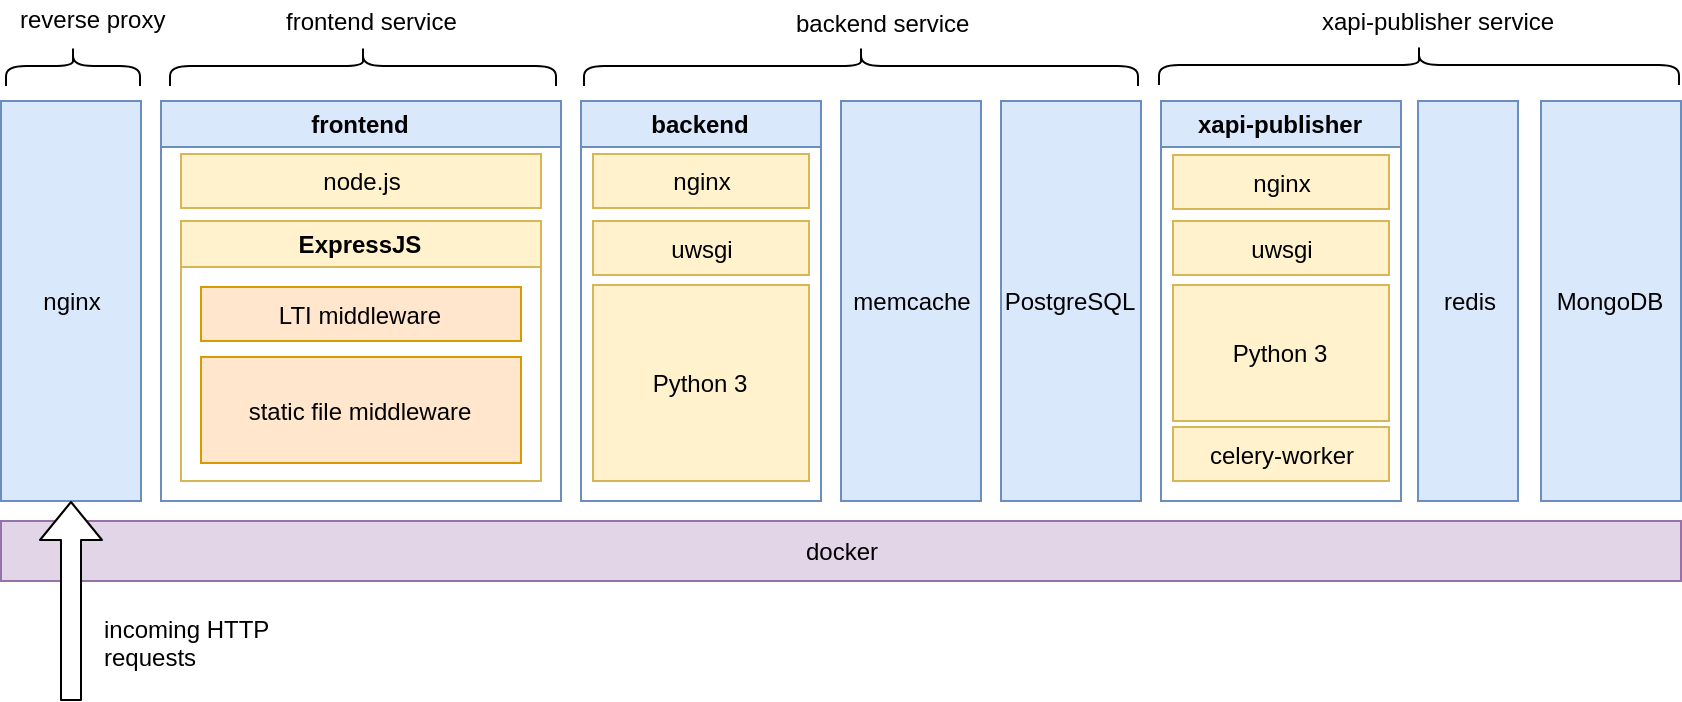
\includegraphics[width=\textwidth]{stack}
        \caption{Server-side software stack}
        \label{fig:stack}
    \end{figure}

    The server-side architecture is composed of multiple services.
    The ``frontend'' service is responsible for serving the
    user interface statically and intercepting LTI requests.
    The ``backend'' service is responsible for serving the API,
    user and session management and communication with the database.
    The ``xapi-publisher'' service is responsible for transmission
    of xAPI statements generated by the backend service.
    Each service uses slightly different technologies, depending
    on the requirements of the service. The API and ``frontend'' service
    are exposed through an nginx web server, which acts as a reverse
    proxy, forwarding incoming HTTP traffic to the appropriate docker
    containers.

    \subsubsection{The Backend Service}
        The backend service is implemented using the Flask
        library, which allows Python to interface with a web server
        using the web server gateway interface \cite{pep-333}. Similar
        to PHP or CGI extensions, the nginx web server will accept incoming
        requests. It will then, using uWSGI, fork a python interpreter
        which will respond to the request. This means that no data
        can be persisted in the Python application itself, as the
        Python context will be discarded for every request.
        To persist data, a PostgreSQL database and a memcached
        in-memory key-value store are used.
        Persistent data, such as survey content, is stored
        in the database, whereas semi-persistent data, such as user
        sessions, is stored in memcached. This design allows
        for horizontal scalability, as multiple instances of the
        \inline{backend} container can be used with the same database.
        No data dependencies exist between the \inline{backend} containers.
        The only bottleneck in this scenario is the shared database.
        This could be solved in the long-term by replacing the single PostgreSQL
        instance by a database cluster.

    \subsubsection{The Frontend service}
        The frontend service consists of a simple node.js
        application running the ExpressJS web server. For the
        web server, two middlewares are provided, one for
        serving static files and another for intercepting LTI launches.
        This is necessary as the user interface has to be
        parameterized for each LTI launch before serving it to the data client.

    \subsubsection{The xAPI-Publisher Service}
    \label{implementation:architecture:xapi-publisher}
        The xapi-publisher service closely mimics the design of the
        backend service. In addition to Flask and uWSGI,
        it also runs several worker threads, which are responsible for the
        asynchronous sending of xAPI statements. Since xAPI statements
        are JSON documents, a document based database - MongoDB - is used instead
        of a relational database to persist xAPI statements between requests.
        For inter-process communication between web server and
        worker threads, a task queue consisting of the Celery library
        and the redis in-memory database is used.

        \begin{wrapfigure}{o}{.5\textwidth}
            \centering
            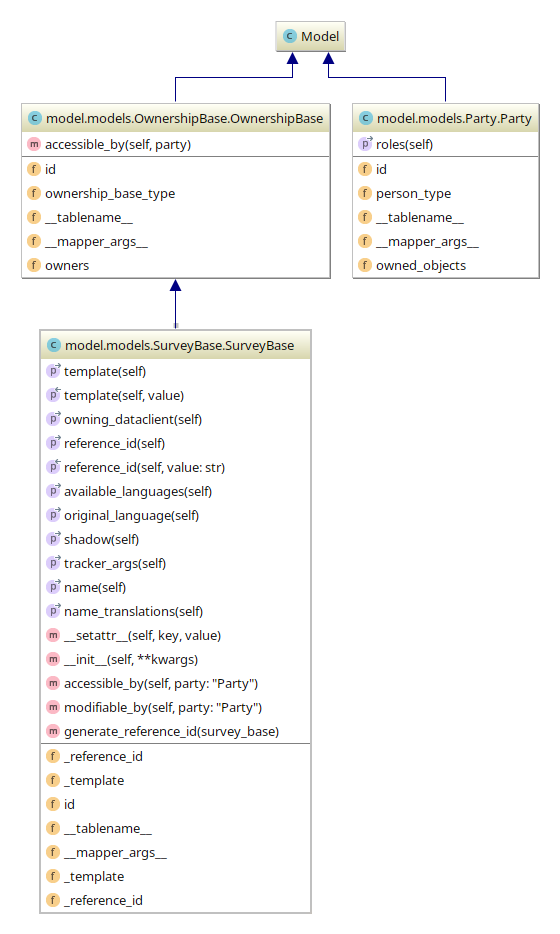
\includegraphics[width=0.49\textwidth]{base-classes}
            \caption{The three main base classes}
            \label{fig:base-classes-dia}
        \end{wrapfigure}

        The functionality provided by the xapi-provider service
        is separate from the backend service, duplicating
        most of the architecture already present. This might at first seem
        less than optimal, as it violates the DRY (don't repeat yourself)
        principle to the extent that configuration for two separate containers
        has to be created and maintained. It does, however, allow for better
        separation of concerns. The backend container already
        handles business logic and user management. A unique
        set of challenges exists that has to be solved for publishing xAPI
        statements, which would unnecessarily increase the complexity
        of the backend service. One such challenge is that
        data needed to create an xAPI statement is sometimes present in a request
        before the data is actually valid and should be transmitted. 
        When a data subject answers a survey using the stand-alone survey
        interface, their answers are submitted to the server but only
        become valid once they have verified their email address.
        The required data to build the xAPI statement, including the data
        subject's IP address, has to be stored on the server until this
        point. In order to avoid convoluting the backend service's
        data model and business logic to account for this, a separate
        service solely responsible for temporarily storing and safely 
        transmitting the xAPI statement is used.
        This allows the backend service to only use minimal logic
        for communicating with the xapi-publisher service.
        It also allows maintainers of the codebase to make changes
        to the publishing behaviour without having to know the internal
        workings of the backend service.

\subsection{Data Model of the \inline{backend} service}
    \subsubsection{Class Hierarchy}
        The class hierarchy is centered around three abstract base classes,
        \inline{SurveyBase}, \inline{OwnershipBase} and \inline{Party}.
        \inline{OwnershipBase} is the base class used for all classes
        which can be owned by a \inline{Party}. \inline{Party} is
        the base class used for all user-type classes. \inline{SurveyBase}
        is the base class for used for all survey items.
        Each of these classes provides common functionality and
        interfaces to their subclasses.

        \begin{figure}
            \centering
            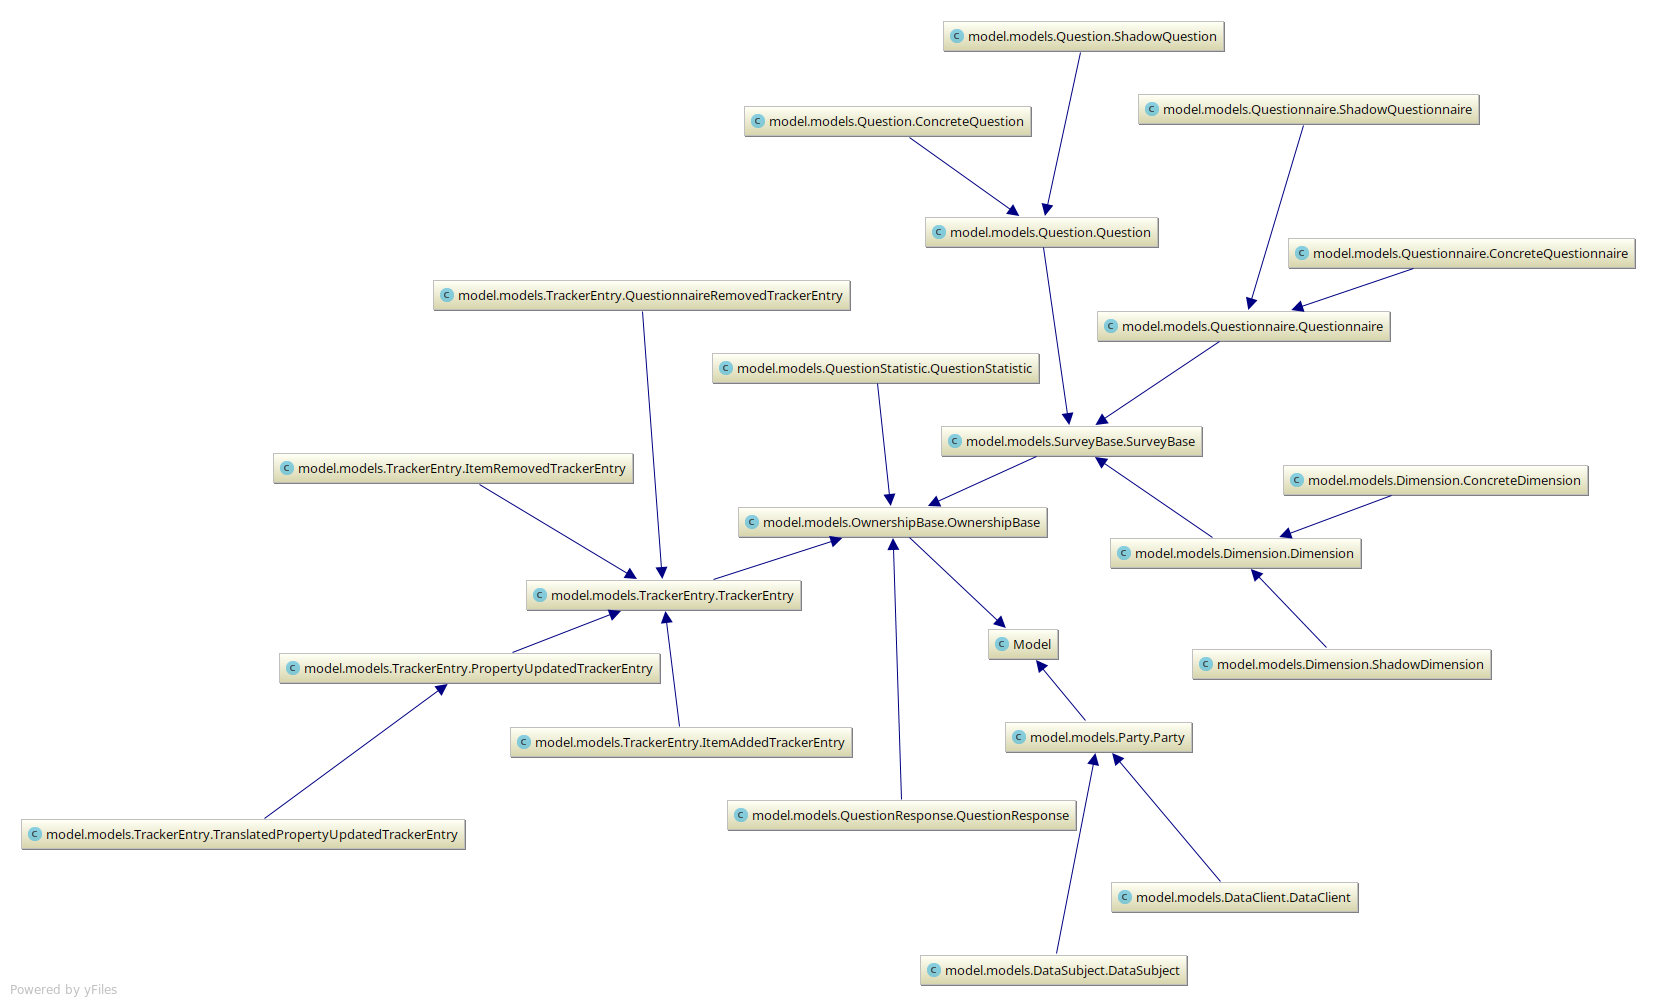
\includegraphics[width=\textwidth]{models}
            \caption{Model class hierarchy}
            \label{fig:model-dia}
        \end{figure}

    \subsubsection{Inheritance Mapping via SQLAlchemy}
    \label{section:implementation:inheritance-mapping}
        The SQLAlchemy library provides three distrinct mechanisms
        for mapping class hierarchies to relational database schemas,
        \textit{joined table inheritance}, \textit{single table inheritance}
        and \textit{concrete table inheritance}.
        Joined table inheritance uses a separate table for every
        class along the hierarchy, with each table only
        containing data declared by the corresponding class.
        Attributes inherited from superclasses are associated
        with subclasses by one-to-one relationships between the
        superclass table and subclass table. When loading
        an instance of a subclass, a join statement is generated,
        which also loads the appropriate record from the superclass
        table. Single table inheritance uses a single table
        for all subclasses of a certain class. Fields
        not used by a certain subclass are populated with \inline{NULL}
        values. Concrete table inheritance uses a separate table for
        every class, which contains all the data needed to load an
        instance of the class. This means that inherited attributes
        will be duplicated in subclass tables.
        From a performance perspective, single or concrete table
        inheritance outperforms joined table inheritance, since
        no join operation is needed to load an instance.
        From a storage perspective, joined table inheritance is
        optimal. Since SQLAlchemy does not support as many
        operations on concrete table inheritance as for the
        other types of inheritance mapping \cite{sqla-inheritance}, concrete inheritance
        mapping was not used. While single table inheritance
        works well for shallow class hierarchies, more
        complex hierarchies with multiple levels of inheritance
        produce only sparsely populated database records, as more attributes
        will be unique than shared for most classes.
        For the survey tool, this approach would only create
        two tables. For storage optimization, the joined
        inheritance approach was used.

    \subsubsection{Template Management - The Template Triad}
    \label{section:implementation:template-triad}
        \begin{figure}
            \centering
            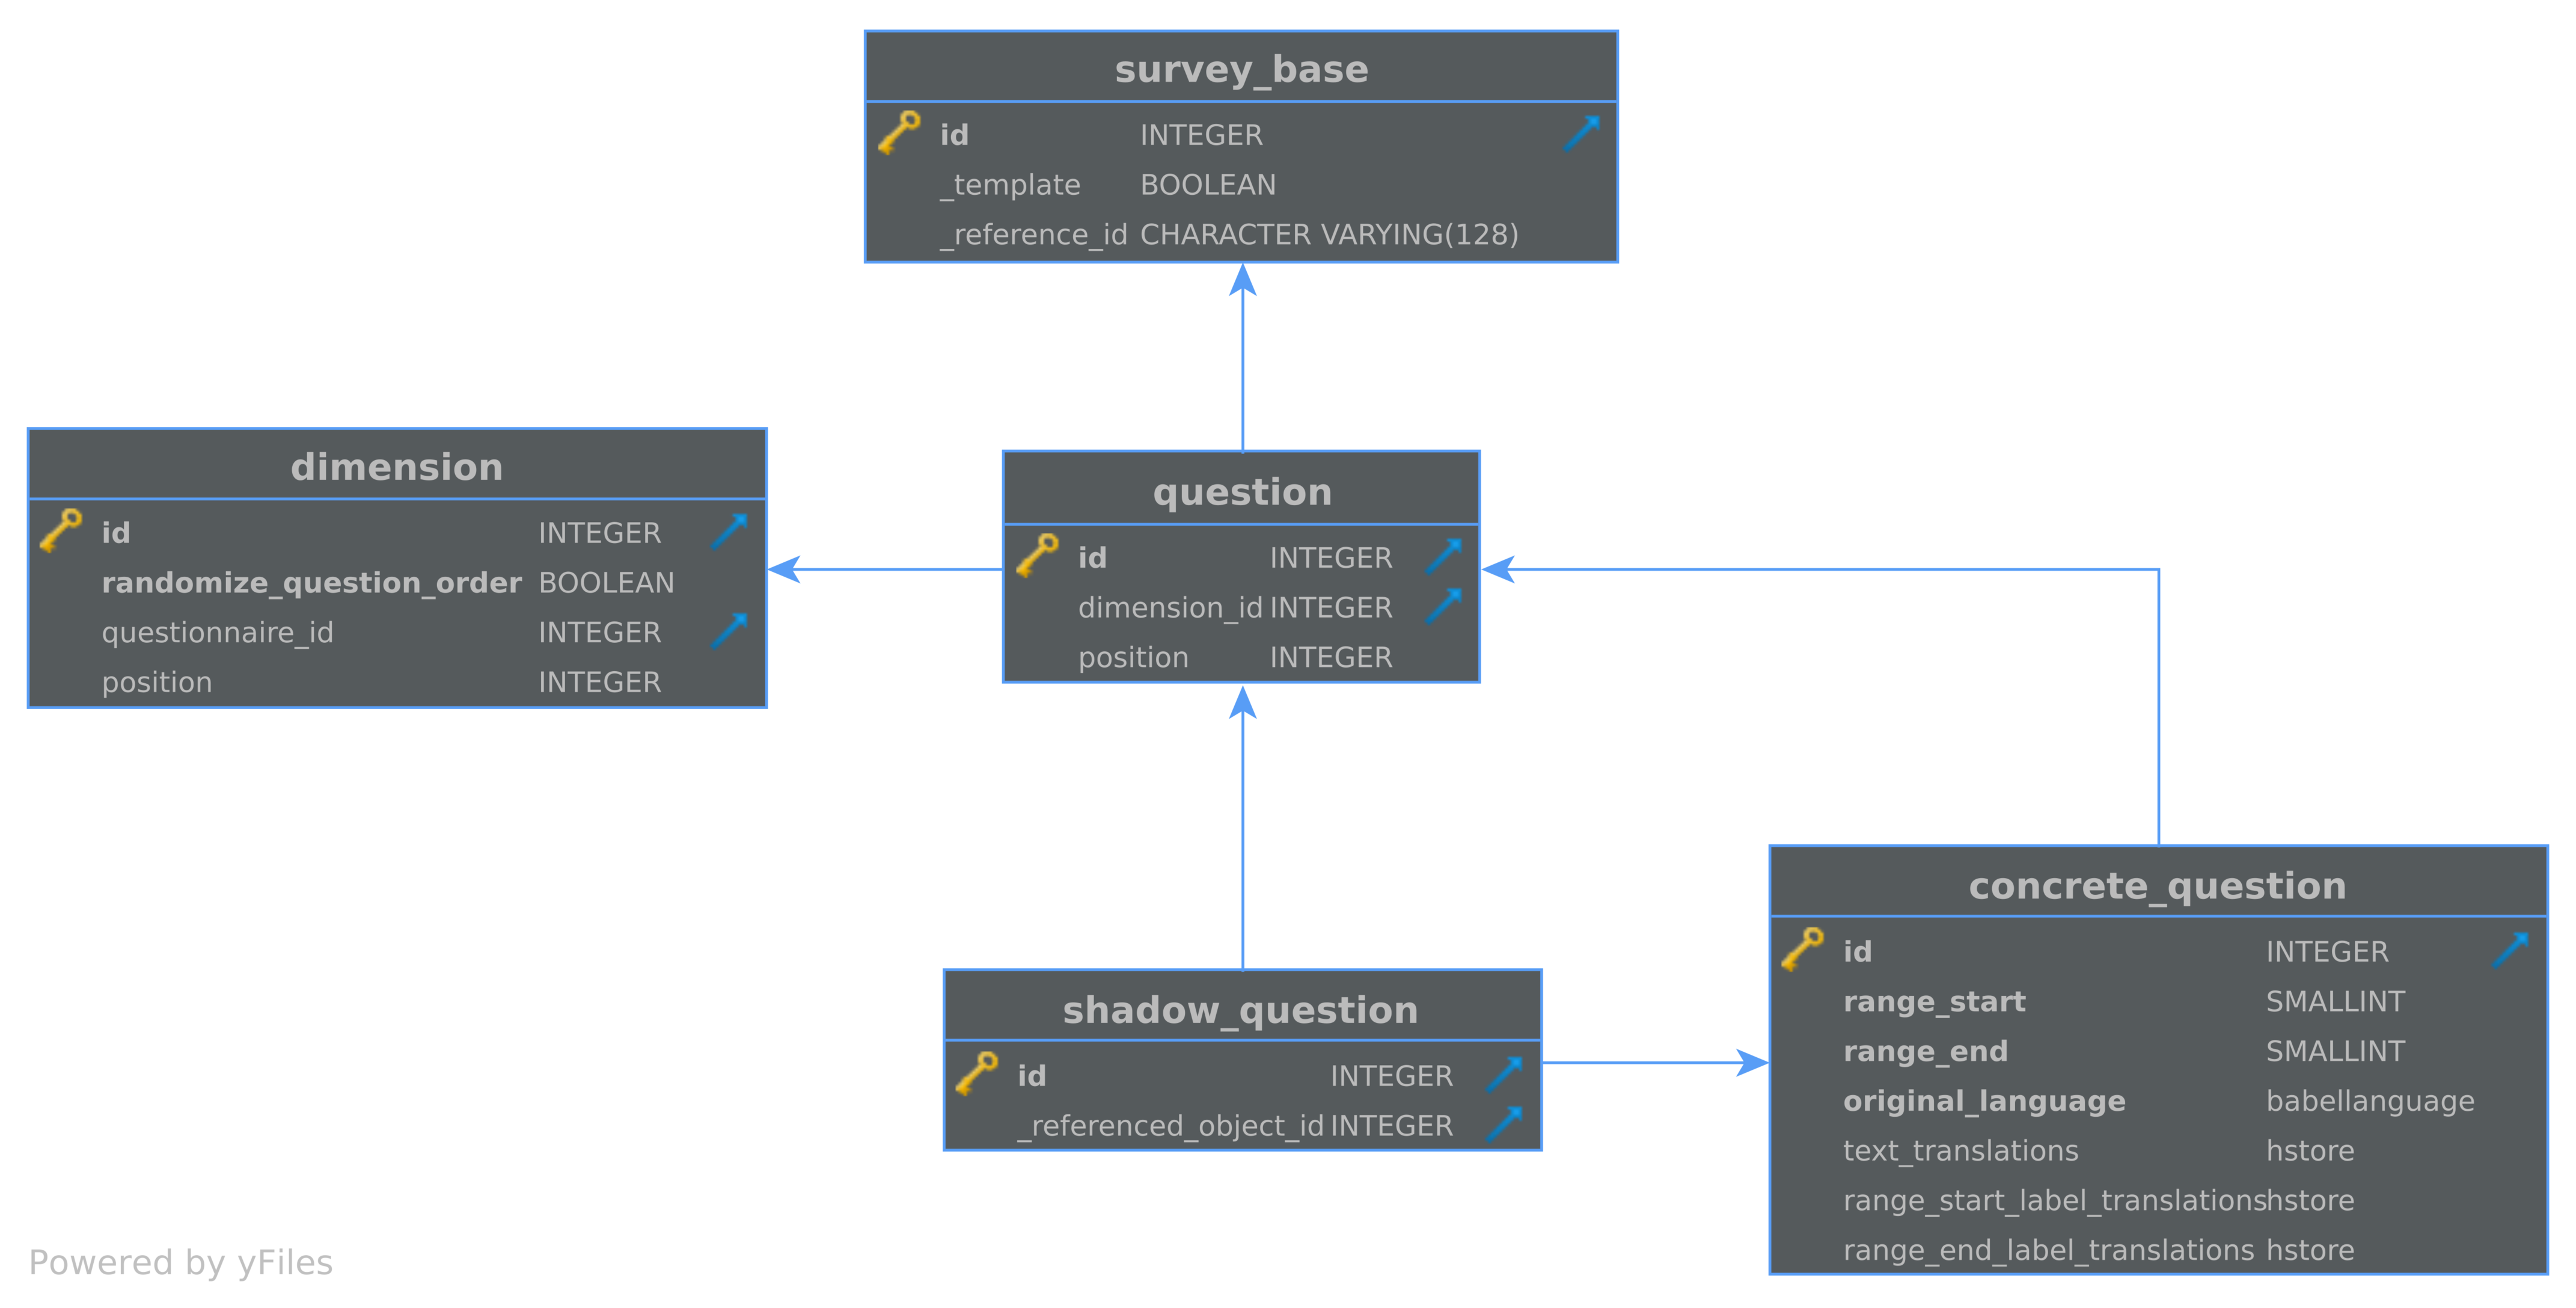
\includegraphics[width=\textwidth]{schema-shadows}
            \caption{Database schema for a single question including foreign key constraints}
            \label{fig:schema-shadows}
        \end{figure}

        To allow user-contributed templates which may also be modified after
        creation, the same data structures are used for templates as for
        regular survey content. Creating copies of these templates is done by
        reference instead of physically copying the template's content.
        This is because template content may be modified
        at any time, and these modifications have to be propagated to
        all existing copies. If copies were created by physically
        copying the template's content, updating a template would
        also cause all copies to be updated in the database. The
        asymptotic number of block accesses of this approach scales linearly
        with the number of copies present and potentially produces
        join operations with large result sets. It also stores
        large amounts of redundant data.Copies, though, are
        proxy objects, which delegate read operation to the referenced
        template. Survey items containing actual data are called
        concrete instances, whereas copies which do not contain
        the actual data are known as shadow instances.
        For each direct \inline{SurveyBase} subclass, \inline{Questionnaire}, \inline{Dimension}
        and \inline{Question}, there are two more subclasses for the concrete and shadow
        representations of the class. this \textit{template triad} is depicted in 
        Figure \ref{fig:questionnaire-dia} and \ref{fig:schema-shadows}. For the sake of brevity,
        the direct descendents of \inline{SurveyBase} will be called the \textit{super-classes},
        while its descendents will be addressed by \textit{concrete} and \textit{shadow}
        respectively. For template management,
        each of these classes fulfils a specific role. All actual data is stored
        in the concrete- and super-classes, while shadow-classes only
        contain a reference to a concrete. As shown in Figure \ref{fig:questionnaire-dia},
        some data is stored in the super-class instead of the concrete class.
        The reason behind this design is, that some attributes of shadow classes
        may still be modified and should not just reflect the state of the associated
        concrete. An example of this is the access control configuration
        of the \inline{Questionnaire} class. Data stored in the concrete
        class can be categorized as \textit{survey content}, while data
        stored in the super-class can be categorized as \textit{administrative data}.
        The super-class also acts as an interface for the concrete and shadow classes,
        specifying all accessors that should be available for its subclasses.
        The shadow classes act as proxies providing transparent read access to the
        referenced concrete's attributes.

        \begin{figure}[H]
            \centering
            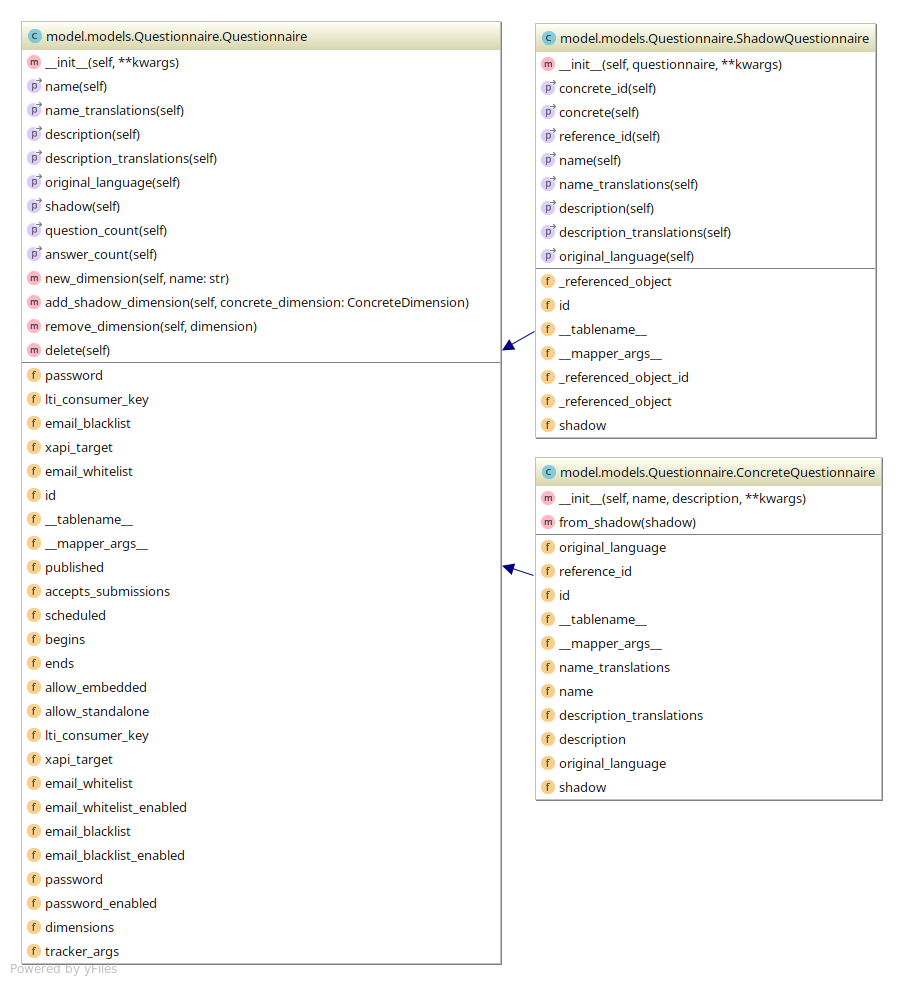
\includegraphics[width=.9\textwidth]{questionnaire-dia}
            \caption{The template triad, exemplarily depicted by the questionnaire data model}
            \label{fig:questionnaire-dia}
        \end{figure}

        \pagebreak

        \begin{wrapfigure}{o}{.5\textwidth}
            \centering
            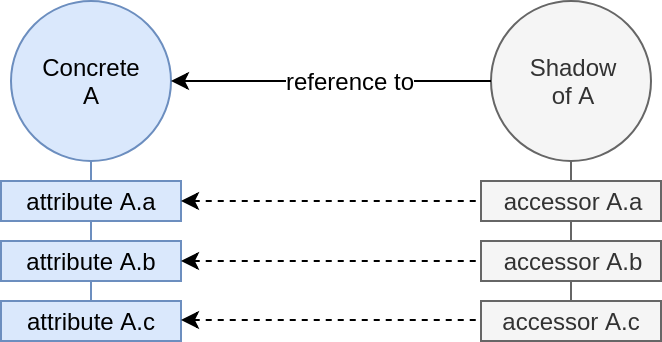
\includegraphics[width=.48\textwidth]{shadow-concept}
            \caption{Schematic depiction of the relationship between concrete \& shadow instances}
            \label{fig:shadow-concept}
        \end{wrapfigure}

\subsection{Template Management}
\label{implementation:template-management}

    \subsubsection{Creation of Shadow Instances}
        Creating a shadow instance from a concrete instance not having
        any relationships to other items is trivial.
        When creating a shadow instance from a concrete instance
        which has children, the resulting shadow
        instance should also duplicate the relationship structure
        of the reference concrete instance. In Figure \ref{fig:concrete-shadow},
        an example for this is given. In the example, Shadow A
        was created from Concrete A. Parent-child relationships
        are modeled as a directed graph with edges from parent to child for the 
        purpose of this example. The creation of Shadow A will cause the
        entire subtree starting from concrete A to be duplicated
        with shadow instances, pointing to their corresponding
        concrete counterparts. The result is a copy of the
        concrete instance and its relationship, which is always
        in synchronism with its source, but can not be modified.

        \begin{wrapfigure}{o}{.6\textwidth}
            \centering
            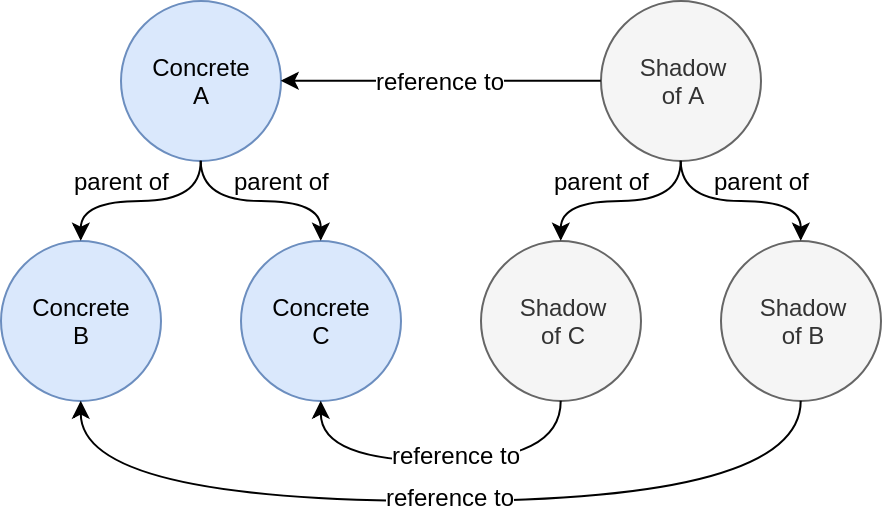
\includegraphics[width=.58\textwidth]{concrete-shadow}
            \caption{Shadow instances duplicate the structure of the concrete items}
            \label{fig:concrete-shadow}
        \end{wrapfigure}

        A special case occurs, when a shadow is created from
        a concrete, whose subtree also contains shadows.
        While it would be possible for a shadow instance to reference another
        shadow instance, a shadow instance should always reference a concrete
        instance directly. The reason for this is the asymptotic number
        of block accesses needed to read from shadow instance. If a shadow references
        another shadow, the \inline{reference_to} relationship would
        have to be traversed multiple times until the concrete instance
        is found. Access times would then scale linearly with
        the degree of separation between the accessed shadow instance
        and the referenced concrete. To avoid this, if a shadow
        instance is encountered while traversing a concrete's
        subtree on shadow creation, the shadow's \inline{reference_to}
        relationship is traversed, until a concrete instance is found.
        The new shadow instance is then created as a reference to this
        concrete instance. The example in Figure \ref{fig:template-contains-copies}
        depicts this case. In the example, Shadow A was created from
        Concrete A. Concrete A's subtree contains a Shadow instance,
        Shadow \#1 of B, which should be duplicated in Shadow A's subtree.
        Instead of pointing Shadow A's right child to concrete A's left child,
        Shadow \#1 of B's \inline{reference_to} relationship is followed.
        Concrete B is encountered
        and becomes the referenced template for shadow \#2 of B.
        This approach maintains the degree of separation between shadows
        and concretes always at one.

        \begin{figure}[H]
            \centering
            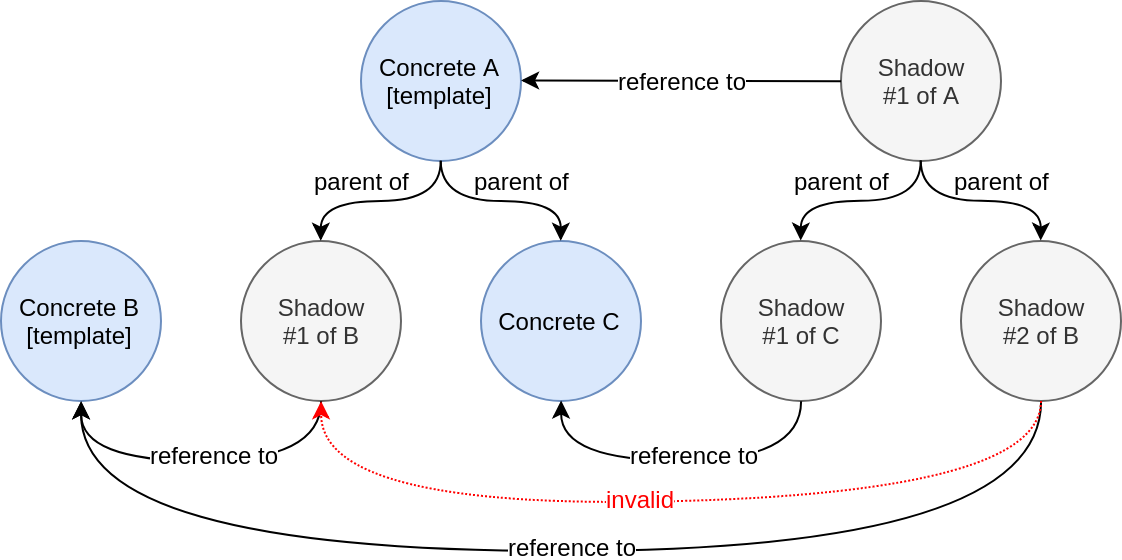
\includegraphics[width=.9\textwidth]{template-contains-copies}
            \caption{Duplication of a concrete structure which contains shadow instances}
            \label{fig:template-contains-copies}
        \end{figure}

    \subsubsection{Modification of Templates}
        Modifications of template content is trivial, as shadow instances
        will always read from the referenced template.
        When modifying a template's relationships to it's children,
        the changes have to be duplicated in all copies of the template.
        To achieve this, the \inline{reference_to} relationship is
        traversed backwards to find all copies of the template. The
        copies are then notified of the modification and apply
        it to their children as well. This operation is
        depicted in Figure \ref{fig:modify-concrete-structure}.

    \subsubsection{Deletion of Templates}
        When a template is deleted, copies of it become invalid,
        as they no longer have any instance to point to.
        Two possible solutions for this are either deleting
        all associated shadows, or converting all associated
        shadows into concrete instances. 
        The former is less complex from an implementation perspective, while the 
        latter is more user-friendly, as it does not result in unexpected 
        deletion of content. There are also use cases, where
        deleting all associated shadows might be intended,
        say, if the survey item is retracted
        and should no longer be used. There is no
        default behavior to satisfy all use cases.
        For this reason, a compromise between the two
        approaches was made. By default, when a template
        is deleted all associated shadows are also deleted.
        Contributors are therefore encouraged to edit existing
        templates instead of deleting them. Templates
        will also show a counter showing the number of
        associated shadows in the user interface, making the
        contributor aware of possible repercussions.
        If the contributor chooses to delete a template anyway,
        the modification tracking feature will provide
        accountability and transparency to the affected data clients.
        When deleting a template questionnaire, however, the
        associated shadows are converted into concrete instances,
        as the questionnaire might already be published and
        available for participation. In this case, deleting
        the questionnaire would interfere with another data
        client's survey and delete already collected results,
        which is not acceptable.

                \begin{wrapfigure}{o}{.7\textwidth}
            \centering
            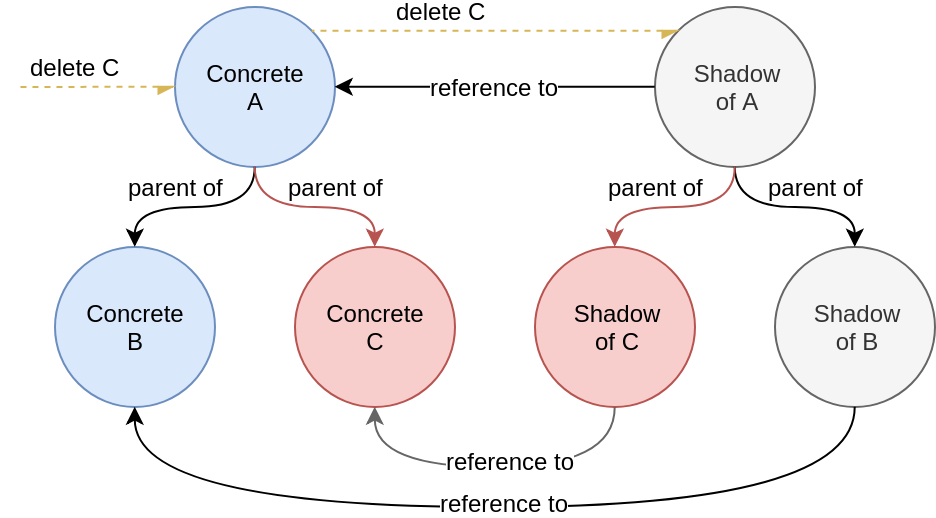
\includegraphics[width=.68\textwidth]{modify-template-structure-delete}
            \caption{Modifications of templates are relayed to copies. Items marked in red are deleted.}
            \label{fig:modify-concrete-structure}
        \end{wrapfigure}

        \begin{figure}[H]
            \centering
            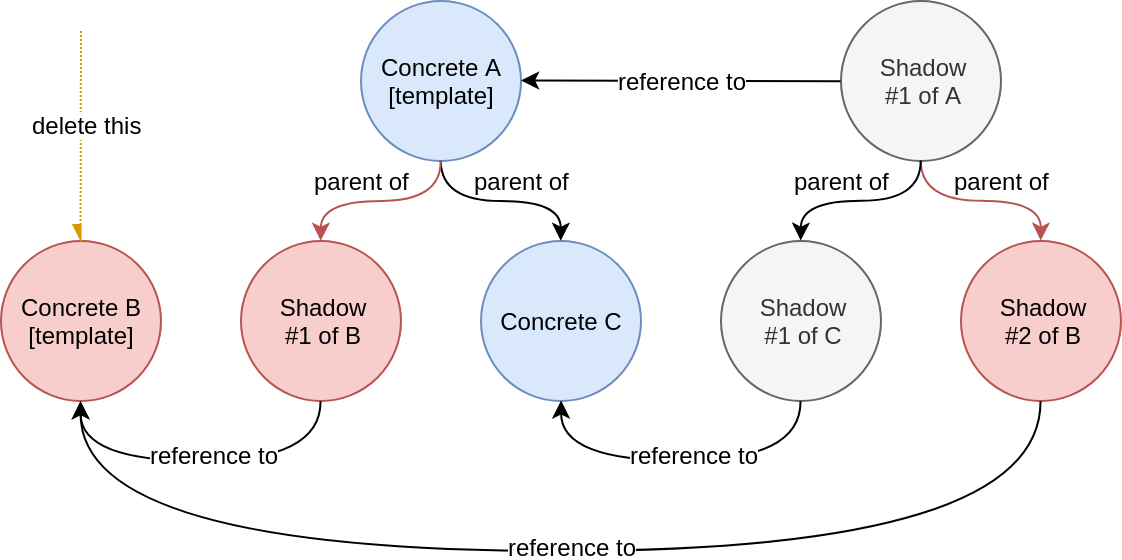
\includegraphics[width=.9\textwidth]{delete-template}
            \caption{Deletion of a template is propagated to all associated shadow instances. Items marked in red are deleted.}
            \label{fig:delete-template}
        \end{figure}

    \subsubsection{Modification Tracking for Templates}
        The modification tracker for a given data client should not 
        merely show changes to concrete instances which are owned by
        the data client. Rather, it should also include changes
        made to templates, of which the data client owns copies of.
        This provides accountability and transparency to data clients
        who choose to use templates. As changes are immediately applied
        to copies, this is an important feature for consistent user
        experience. To achieve this, every time a modification
        is made to a template, ownership of the resulting tracking record 
        is given not only to the template owner, but to all
        owners of associated shadow instances.

\subsection{API}
    The API is organized using the \inline{Flask-RESTful}
    library \cite{flask-restful}. For each type of survey item, a canonical endpoint and a set of
    contextual endpoints exist, all of which are mapped to the same handler.
    Canonical endpoints follow the \inline{http://HOST:PORT/api/TYPE/ID} format,
    where \inline{TYPE} is the type of survey item. Each survey item is identified
    by it's unique ID, which may be used for accessing the item via its endpoints.
    If a survey item has child elements, then these may be accessed by
    appending \inline{/CHILD_TYPE/} or \inline{/CHILD_TYPE/CHILD_ID} to any
    of the parent's endpoints. The former returns a list of all children,
    while the latter accesses a single child. These endpoints are called
    contextual endpoints.

    Each survey item is also associated with at least one JSON schema,
    which is used for serialization and deserialization of the classes
    instances. The schemas are implemented using the Marshmallow
    library. Each survey item's schema also includes a URL pointing to
    the canonical endpoint of the item, which may be used for
    fetching the item again in the future.

    Before any other request handler is invoked in the backend,
    information about the request language and user session are parsed.
    The request locale is determined by three mechanisms, which take
    precedence over each other in the order mentioned here
    (the latter overrides the former). First, the HTTP headers
    are inspected for the \inline{Accept-Languages} field and the best
    match is chosen from the list of available languages.
    If cookies were sent with the request, they are searched for
    a \inline{locale} cookie. Lastly, the request parameters
    are inspected for the \inline{locale} parameter.
    Session information is communicated using the \inline{Authentication}
    field of the request headers, following the bearer authentication scheme.
    If a session token is found in the HTTP headers, the token is validated.
    If successful, the associated \inline{Party} object is loaded and
    injected into the request context.    

\subsection{Authentication}
    \subsubsection{Data Client Authentication}
        Authentication for data clients can be performed by providing
        a valid combination of email and password. These parameters
        are sent to the backend in JSON format. The request
        can be encrypted by the client using TLS when a valid
        certificate is provided for the load balancer. The load balancer
        will then decrypt the request and pass it unencrypted to the backend
        on the virtual network. When creating a new data client,
        a random salt is generated using the operating system's
        random device. The provided password and salt are then hashed
        using the native Python implementation of the Argon2 password hashing function \cite{argon2}.
        The password hash and salt are stored in
        the database and can be used to validate login attempts
        by re-applying the hashing algorithm to the salt and the provided
        password, and comparing the resulting hash with the stored hash.

    \subsubsection{Session Management}
        Once a \inline{Party} has been successfully authenticated, a \textit{session record}
        is created and published to the \inline{memcached} instance.
        This session record includes information about the
        \inline{Party}, a timestamp of the last performed action by the \inline{Party}
        and a randomly generated \textit{session token}.
        The session token is handed out to the client via the API
        and may be used by the client to identify itself
        in subsequent requests. Every time the session token is used
        in a request, the timestamp stored in the session record is
        updated to the current time. If the difference between
        the timestamp and the current time exceeds a certain limit
        in any request, the token is rejected and the session record
        is removed from \inline{memcached}. This ensures the eventual
        removal of unused session records from the cache and protects
        the user against re-use of their session token if they forgot
        to log out. Another protection against token stealing
        is IP pinning. When a user is successfully authenticated,
        their IP address is included in the session record.
        If any subsequent request with the associated token
        uses a different IP address than was used for authenticating,
        the token will be rejected and the session will be removed
        from the cache.

        \begin{wrapfigure}[20]{o}{.5\textwidth}
            \centering
            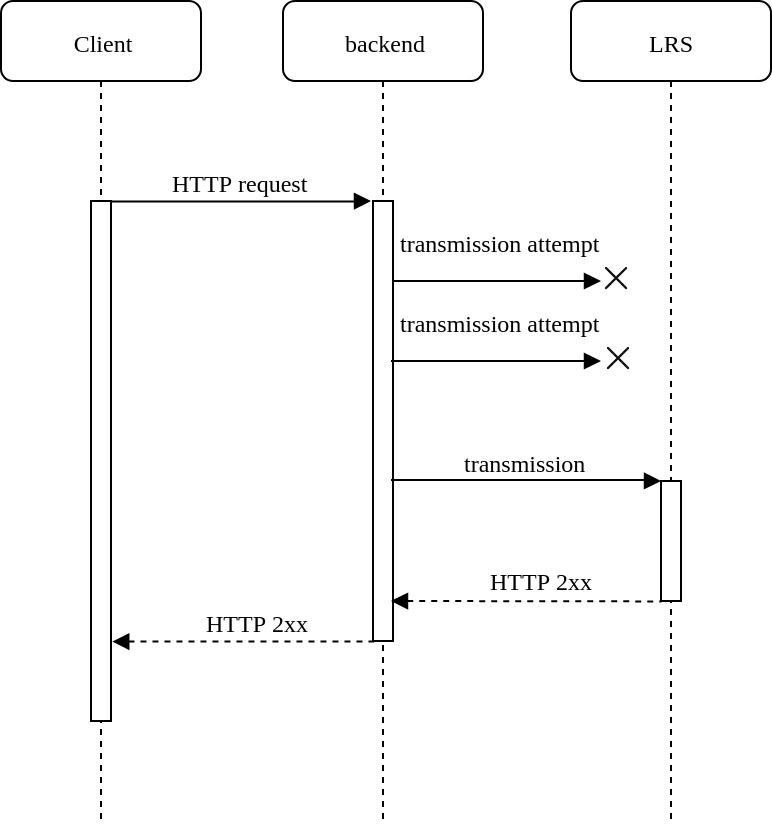
\includegraphics[width=.48\textwidth]{synchronous-xapi}
            \caption{Synchronous (blocking) transmission of xAPI statements}
            \label{fig:synchronous-xapi}
        \end{wrapfigure}

\pagebreak

\subsection{Support for xAPI}
\label{implementation:xapi}
     
    \subsubsection{xAPI in the Backend Service}
        xAPI statements are created in the backend service using an
        object-oriented API. Statements are queued locally using
        the \inline{XApiPublisher} class, which acts as a transaction manager
        for xAPI statements. When a request context is created by the
        WSGI middleware, a new transcation is started. 
        Queued statements are only sent to the \inline{xapi-publisher} service, 
        when the transaction is committed at any point during handling 
        of the request. By default, when the request was handled
        without raising an error, and a rollback was not explicitly
        executed during the request, the transaction is committed automatically
        at the end of the request.

    \subsubsection{The xAPI-Publisher Service}

        \begin{figure}
            \centering
            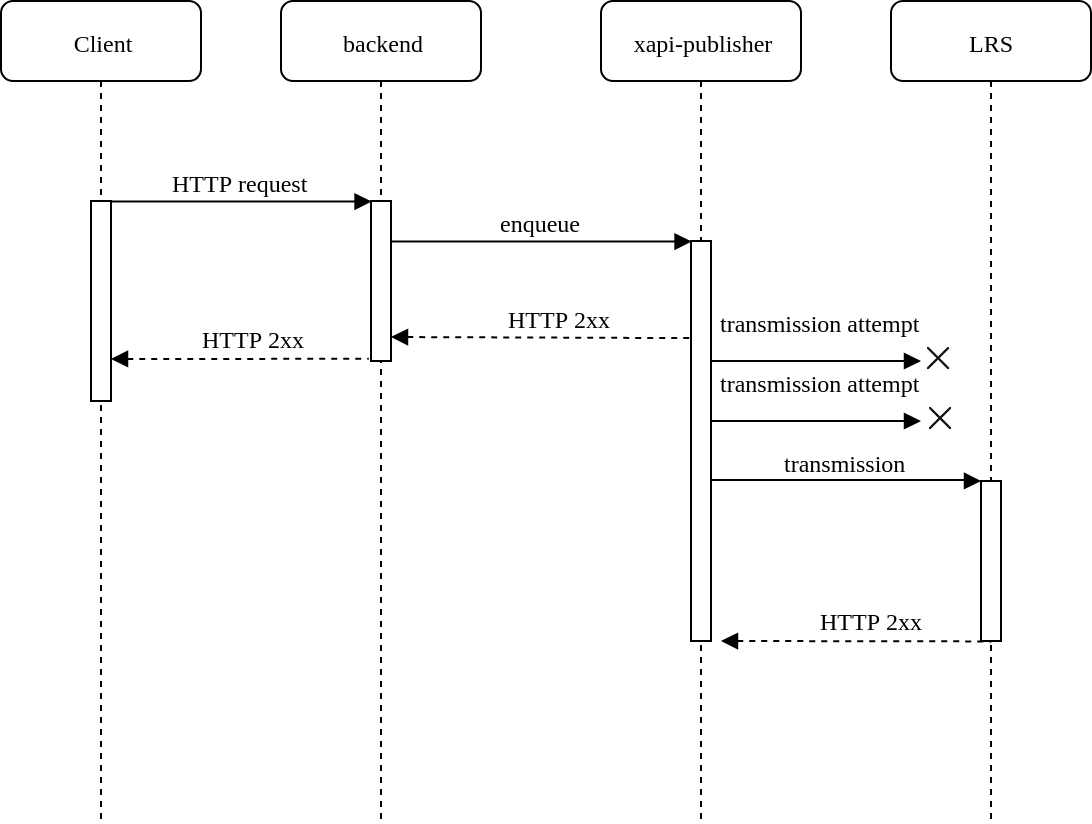
\includegraphics[width=.8\textwidth]{asynchronous-xapi}
            \caption{Asynchronous (non-blocking) transmission of xAPI statements}
            \label{fig:asynchronous-xapi}
        \end{figure}

        Sending of xAPI statements is separated from the API, as sending and
        possible re-transmissions should not block the API from responding
        to requests. This was discovered during testing, when a misconfigured xAPI
        recipient was used. HTTP timeouts are usually in the order of seconds and 
        unsuccessful connection attempts are retried. This resulted in
        the site becoming unresponsive when submitting the survey, as the submission
        of a survey would cause a large number of xAPI statements to be sent.
        Figures \ref{fig:synchronous-xapi} and \ref{fig:asynchronous-xapi} illustrate
        this issue.

\subsection{LTI Middleware}
    As mentioned before, recognition of data subjects uses the same token-based
    mechanism that is also used for recognizing data-client sessions.
    Since session management is performed by the backend service,
    but the frontend bundle is served by the frontend service, performing
    an LTI launch involves both services. The frontend provides an HTTP
    endpoint for requesting the LTI launch. The supplied information
    is then forwarded to the backend service, which validates
    the supplied combination of consumer key and requested questionnaire.
    If the LTI launch is valid, the backend service starts a new session
    for the data subject. A session token is then returned to the frontend
    service. The frontend service embeds the session token as a global
    variable into the JavaScript bundle which is the user interface and
    serves the parameterized bundle to the client.
    The user interface's bootstrapping process may then check for
    the presence of the session token and switch to it's embedded version.
    The embedded version of the user interface uses a different endpoint
    for submitting responses than the standalone version, as no information
    about the data subject has to be present in the response.
    A sequence diagram for the LTI launch is provided in Figure \ref{fig:lti-launch}.

    \begin{figure}
        \centering
        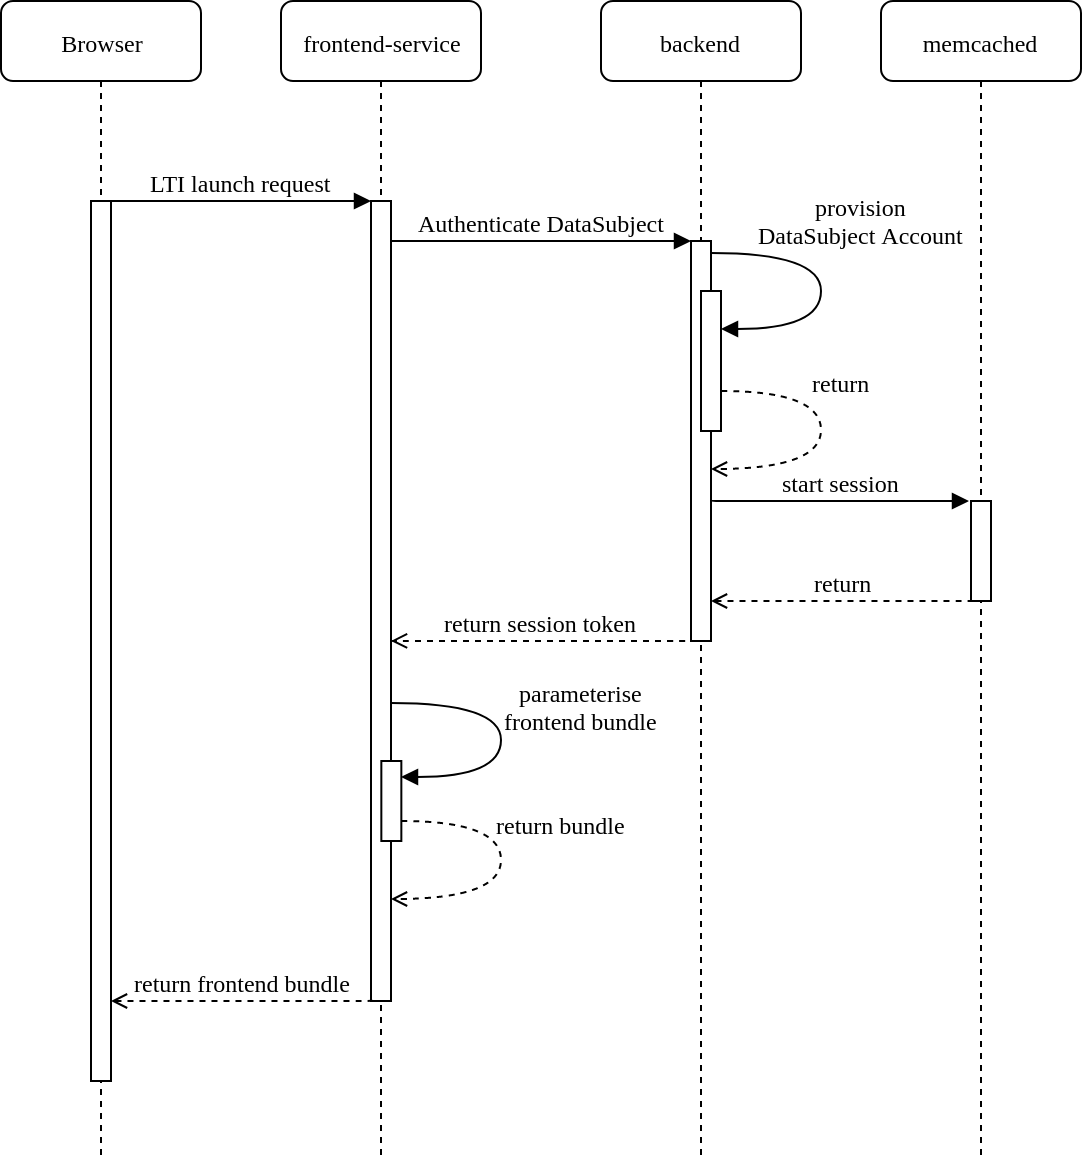
\includegraphics[width=.85\textwidth]{lti-launch}
        \caption{Sequence diagram depicting the LTI launch}
        \label{fig:lti-launch}
    \end{figure}
    
